\section{Generation of a porous matrix}
Our plan to generate a porous material is to first generate a thermalized Lennard-Jones system, and then select a given part of the sytem to be the solid matrix. The simplest version is to freeze all the atoms in the matrix, 
meaning they are not allowed to move, but still let them interact with the particles that are allowed to move. One way to make pores is to generate randomly large spheres placed at random in the Lennard-Jones liquid,
and choose to let the particles inside the spheres be frozen, or the other way around.
\subsection{Cylindrical pore}
To practice our pore-making-skills, the first task was to make a cylindrical pore with radius $R=2nm$ at the center of a system with $N_x=N_y=N_z= 20$ unit cells of size $b=5.72 $A. First, the system
is thermalized at $T = 0.851T_0 = 101.9K$. I made the matrix by letting the atoms know if they are able to move, or not. They all have an attribute called canMove, which is boolean true if the atom in fact is able to move.
After thermalizing the system, I marked the particles outside the cyllinder by setting ``canMove`` to ''false``. Then, only the particles that are unable to move are written to a VMD-file (my program can also do it the other way around).
In figure \ref{cyllinder} we have a visualization of the matrix.
\begin{figure}[H]
 \centering
 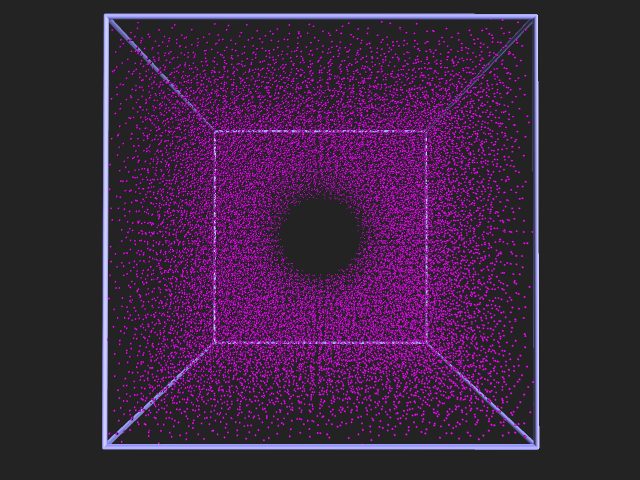
\includegraphics[width=12 cm]{./figures/cyllindircal_pore.png}
 % cyllindircal_pore.png: 640x480 pixel, 96dpi, 16.93x12.70 cm, bb=0 0 480 360
 \caption{A cylindrical pore of radius $R = 2$ nm. The length of the system in each space direction is $20\cdot 5.72\text{A} = 11.44 $nm}
 \label{cyllinder}
\end{figure}

\subsection{First nano-porous system}
In figure \ref{pores_20} you see the argon liquid with 20 pores at random positions. The white particles are atoms that are not able to move. I have not yet time evolved the system.
\begin{figure}[H]
 \centering
 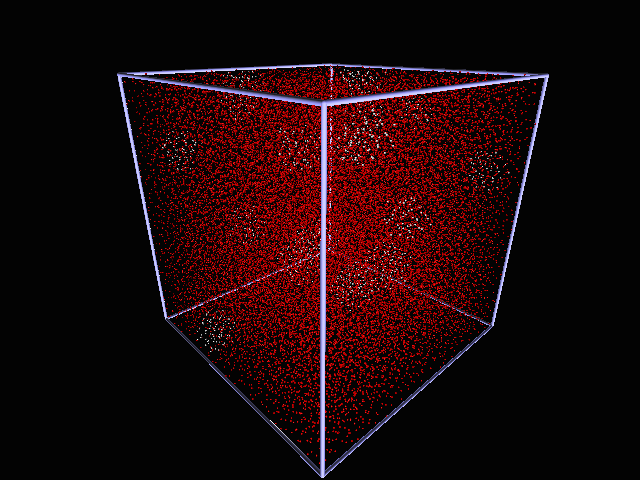
\includegraphics[width=12 cm]{./figures/pores_20.png}
 % pores_20_done.png: 1850x1157 pixel, 96dpi, 48.94x30.61 cm, bb=0 0 1387 868
 \caption{Argon liquid with 20 randomly sized and placed pores.}
 \label{pores_20}
\end{figure}

We can see here that the matrix constitute a small amount of the total volume, which is a bit counter intuitive to me. I decided to increase the number of spheres to 100, and found that 
the matrix looks more reasonable, see figure \ref{pores_100}.
\begin{figure}[H]
 \centering
 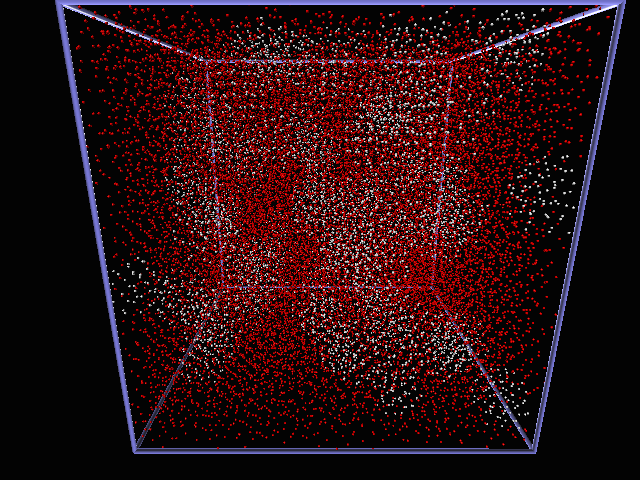
\includegraphics[width=12 cm]{./figures/pores_100.png}
 % pores_20_done.png: 1850x1157 pixel, 96dpi, 48.94x30.61 cm, bb=0 0 1387 868
 \caption{Argon liquid with 20 randomly sized and placed pores.}
 \label{pores_100}
\end{figure}

\subsection{Porosity}
The porosity, $\phi$, is the relative amount of pore space in the volume. To calculate this I first found the average volume of each atom by dividing the total volume by the number of 
particles, before cutting out the pores. Then I just counted all the particles set as unmovable, and multiplied this number by the average volume to find the volume of the matrix.
\begin{align}
 V_a = V/N_{all}\nonumber\\
 V_{matrix} = V_a N_{matrix}\nonumber
\end{align}
We can now set the porosity as
\begin{align}
 \phi = 1-V_{matrix}/V
\end{align}


 
